
% ----------------------------------------------------------------------
%  Set the document class
% ----------------------------------------------------------------------
\documentclass[11pt,a4paper,twoside]{article}

% ----------------------------------------------------------------------
% Define external packages, language, margins, fonts and new commands
% ----------------------------------------------------------------------
%\input{preamble} 
\usepackage[utf8]{inputenc}   % <<<<< Linux
\usepackage[english]{babel} % <<<<< English
\usepackage{notoccite}
\usepackage[skip=0.5\baselineskip]{caption}
\hyphenation{GTKWave}
\usepackage{listings}
\usepackage[all]{nowidow}

%blind text
\usepackage{lipsum}

\usepackage{graphicx}
\graphicspath{{./}{../../figlib/}{../mat/}{../sim/}}
\def\FontLn{% 16 pt normal
  \usefont{T1}{phv}{m}{n}\fontsize{16pt}{16pt}\selectfont}
\def\FontLb{% 16 pt bold
  \usefont{T1}{phv}{b}{n}\fontsize{16pt}{16pt}\selectfont}
\def\FontMn{% 14 pt normal
  \usefont{T1}{phv}{m}{n}\fontsize{14pt}{14pt}\selectfont}
\def\FontMb{% 14 pt bold
  \usefont{T1}{phv}{b}{n}\fontsize{14pt}{14pt}\selectfont}
\def\FontSn{% 12 pt normal
  \usefont{T1}{phv}{m}{n}\fontsize{12pt}{12pt}\selectfont}

% Use Arial font as default
%
\renewcommand{\rmdefault}{phv}
\renewcommand{\sfdefault}{phv}
\usepackage{geometry}	
\geometry{verbose,tmargin=2.5cm,bmargin=2.5cm,lmargin=2.5cm,rmargin=2.5cm}

%\usepackage{setspace}
%\renewcommand{\baselinestretch}{1.5}

\usepackage[pdftex]{hyperref} % enhance documents that are to be
                              % output as HTML and PDF
\hypersetup{colorlinks,       % color text of links and anchors,
                              % eliminates borders around links
%            linkcolor=red,    % color for normal internal links
            linkcolor=black,  % color for normal internal links
            anchorcolor=black,% color for anchor text
%            citecolor=green,  % color for bibliographical citations
            citecolor=black,  % color for bibliographical citations
%            filecolor=magenta,% color for URLs which open local files
            filecolor=black,  % color for URLs which open local files
%            menucolor=red,    % color for Acrobat menu items
            menucolor=black,  % color for Acrobat menu items
%            pagecolor=red,    % color for links to other pages
            pagecolor=black,  % color for links to other pages
%            urlcolor=cyan,    % color for linked URLs
            urlcolor=black,   % color for linked URLs
	          bookmarks=true,         % create PDF bookmarks
	          bookmarksopen=false,    % don't expand bookmarks
	          bookmarksnumbered=true, % number bookmarks
	          pdftitle={report},
            pdfauthor={Andre C. Marta},
%            pdfsubject={Thesis Title},
%            pdfkeywords={Thesis Keywords},
            pdfstartview=FitV,
            pdfdisplaydoctitle=true}

\usepackage[numbers,sort&compress]{natbib} % <<<<< References in numbered list [1],[2],...
\usepackage{subcaption} 
\usepackage{mdframed}

%%%%%%%%%%%%%%%%%%%%%%%%%%%%%%%%%%%%%%%%%%%%%%%%%%%%%%%%%%%%%%%%%%%%%%%%
%     Begin Document                                                   %
%%%%%%%%%%%%%%%%%%%%%%%%%%%%%%%%%%%%%%%%%%%%%%%%%%%%%%%%%%%%%%%%%%%%%%%%


\begin{document}

% Set plain page style (no headers, footer with centered page number)
\pagestyle{plain}

% Set roman numbering (i,ii,...) before the start of chapters
%\pagenumbering{roman}

% ----------------------------------------------------------------------
%  Cover page
% ----------------------------------------------------------------------
%%%%%%%%%%%%%%%%%%%%%%%%%%%%%%%%%%%%%%%%%%%%%%%%%%%%%%%%%%%%%%%%%%%%%%%%
%                                                                      %
%                                      %
%                                                                      %
%%%%%%%%%%%%%%%%%%%%%%%%%%%%%%%%%%%%%%%%%%%%%%%%%%%%%%%%%%%%%%%%%%%%%%%%

\thispagestyle {empty}

% IST Logo - Signature A
% parameters: bb=llx lly urx ury (bounding box), width=h_length, height=v_length, angle=angle, scale=factor, clip=true/false, draft=true/false. 

\includegraphics[bb=9.5cm 11cm 0cm 0cm,scale=0.29]{IST_A_CMYK_POS}

\begin{center}
%
% Figure (Image or plot)
\vspace{1.0cm}
% height = 50 mm
%\includegraphics[height=50mm]{Figures/Airbus_A350.jpg}

% Title, author and degree
\vspace{1cm}
{\FontLb Circuit Theory and Electronics Fundamentals} \\ % <<<<< EDIT TITLE
\vspace{1cm}
{\FontLb T3} \\
\vspace{1cm}
{\FontSn Physics Engineering, Técnico, University of Lisbon} \\ % <<<<< EDIT COURSE
\vspace{1cm}
{\FontSn May 8, 2021} \\ % <<<<< EDIT DATE (corresponds to date of oral examination)
%
\end{center}



% ----------------------------------------------------------------------
% Dedication page (optional)
% ----------------------------------------------------------------------
%\input{dedication} 
%\cleardoublepage

% ----------------------------------------------------------------------
%  Acknowledgments (optional)
% ----------------------------------------------------------------------
%\input{acknowledgements}
%\cleardoublepage

% ----------------------------------------------------------------------
%  Abstract (both in English and Portuguese)
% ----------------------------------------------------------------------
%\input{resumo} 
%\cleardoublepage

%\input{abstract} 

% ----------------------------------------------------------------------
%  Table of contents, list of tables, list of figures and nomenclature
% ----------------------------------------------------------------------

% Table of contents
%
\tableofcontents

% List of tables
%\addcontentsline{toc}{section}{\listtablename}
%\listoftables
%\cleardoublepage 

% List of figures
%\addcontentsline{toc}{section}{\listfigurename}
%\listoffigures
%\cleardoublepage 

% Set arabic numbering (1,2,...) after preface
%
%\setcounter{page}{1}
%\pagenumbering{arabic}

% ----------------------------------------------------------------------
%  Body
% ----------------------------------------------------------------------

\section{Introduction}
\label{sec:introduction}
\paragraph{}
\par The goal of this laboratory assignment is to study and analyse a RC circuit composed by a dependent current source, a capacitor, resistors, and  lastly, one dependent and one independent voltage source to find the natural and forced response and frequency analysis of the said circuit.
A comparison will be done between the NgSpice simulation and the theoretical analysis of the circuit.
\par The main objective will be to further learn about both methods of analysis, learning about their similarities, differences and which positive and negative sides each of them have. 
\par The circuit is represented with resort to \textit{LibreOffice Draw} and can be viewed in figure \ref{circuit}.

\begin{figure}[H]
    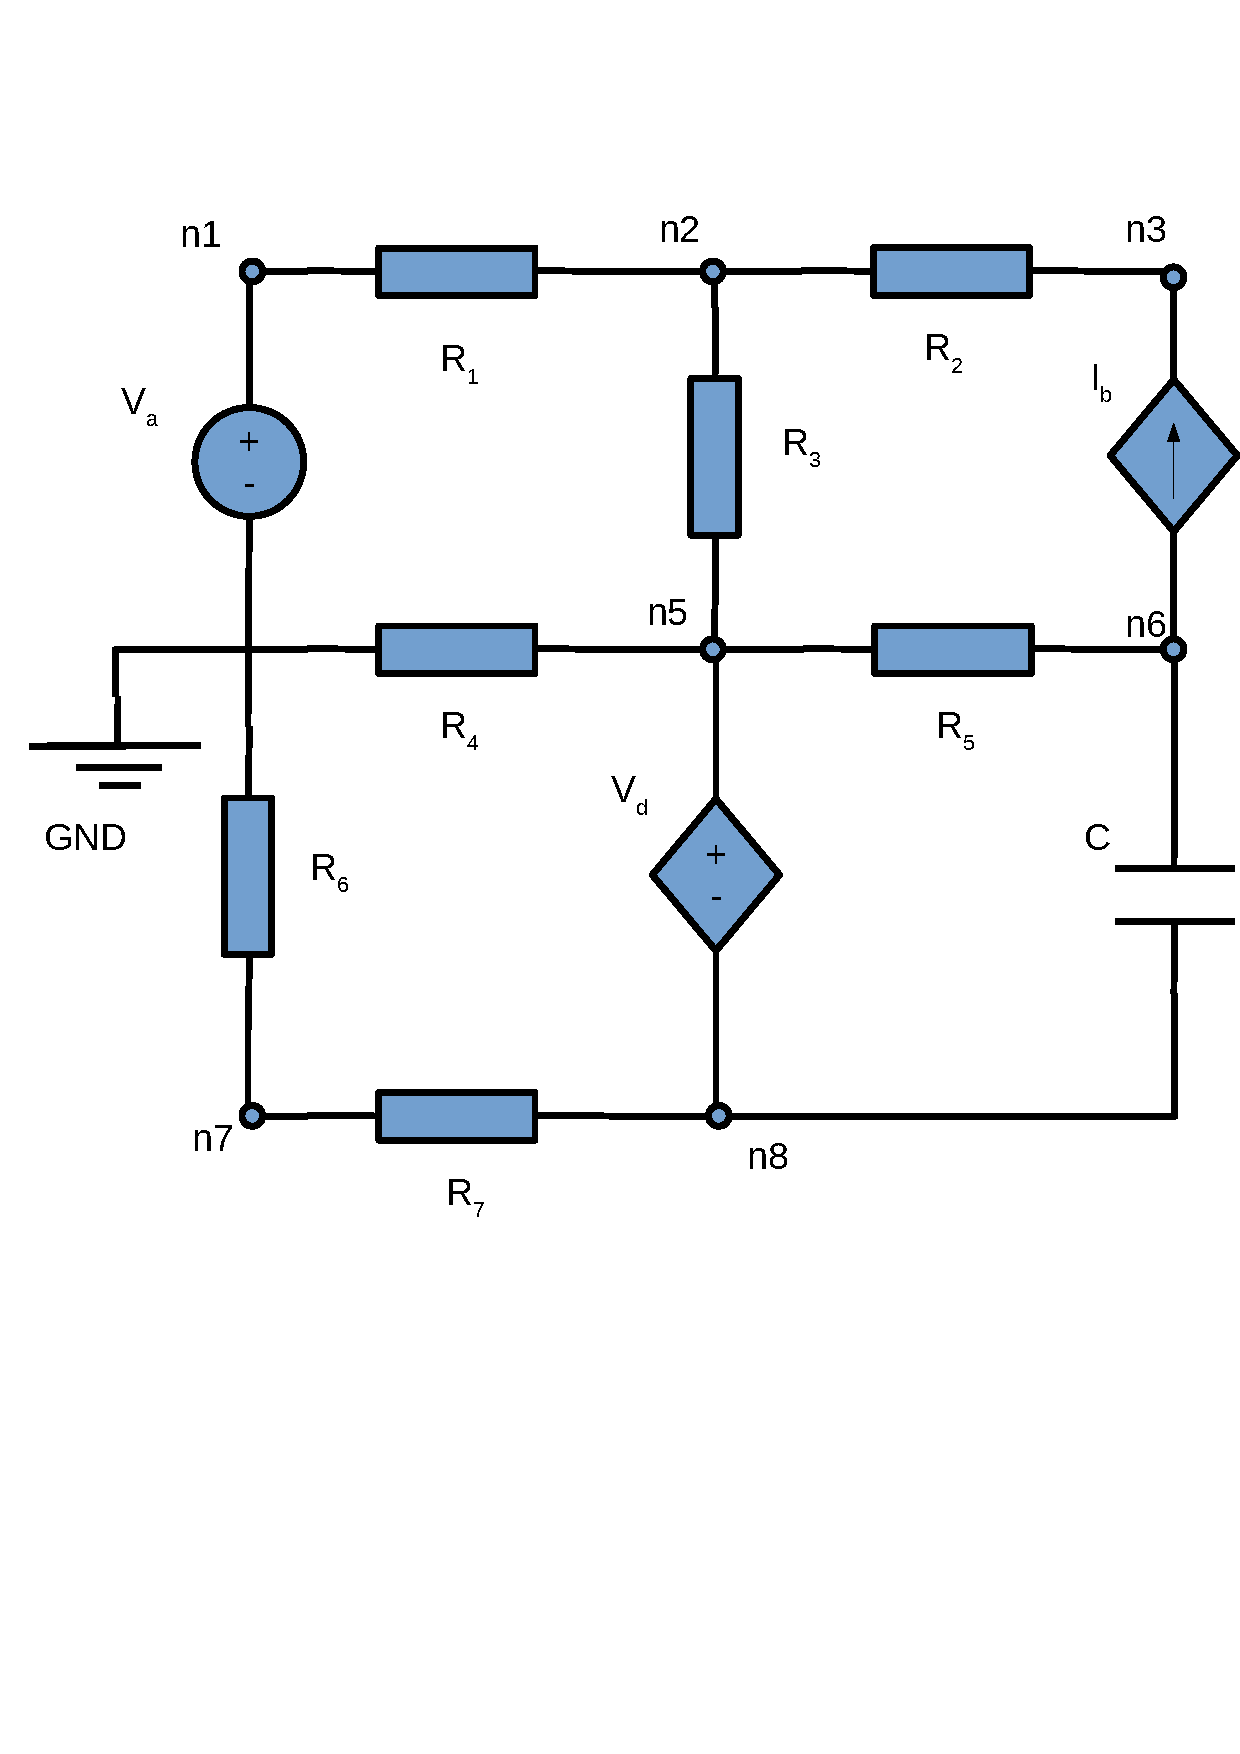
\includegraphics[width=0.5\linewidth]{Lab2.pdf}
    \centering
    \caption{Studied Circuit}
    \label{circuit}
\end{figure}


In Section~\ref{sec:analysis}, a theoretical analysis of the circuit is
presented. In Section~\ref{sec:simulation}, the circuit is analysed by
simulation, and the results are compared to the theoretical results obtained in
Section~\ref{sec:analysis}. The conclusions of this study are outlined in
Section~\ref{sec:conclusion}.


\section{Theoretical Analysis}
\label{sec:analysis}
\paragraph{}

\par In this section, the circuit is analyzed in theory through Octave calculations. The BPF circuit shown in the introduction basically consists of a high pass filter in series with a low pass filter and a signal amplifier. To be able to make calculations, the OpAmp characteristics are assumed to be ideal, that means its impedance is infinite for the input and null for output.
\par With the values for the components given in table 1, it is possible to calculate the following values:

\begin{table}[H]
    \centering
    \begin{tabular}{|c|c|}
    \hline
        \input{../mat/TA.tex}
    \end{tabular}
    \caption{Values for Gain, Input and Output impedances calculated thgrouh Octave}
    \label{TA}
\end{table}

\par Finally the frequency response $V_0(f)/V_i(f)$ is ploted for the gain:

\begin{figure}[H]
	\includegraphics[width=0.5\linewidth]{gain.eps}
	\centering
	\caption{Gain plot - $\frac{V_o(f)}{V_i(f)}$}
	\label{gain}
\end{figure}

\par And for the phase:

\begin{figure}[H]
	\includegraphics[width=0.5\linewidth]{phase.eps}
	\centering
	\caption{Phase plot}
	\label{pha}
\end{figure}


\section{Simulation Analysis}
\label{sec:simulation}
\paragraph{}
\par For this simulation analysis, it is convenient to represent graphically, with  \textit{LTSpice}, the studied circuit, that can be seen in the following figure.

\begin{figure}[H]
    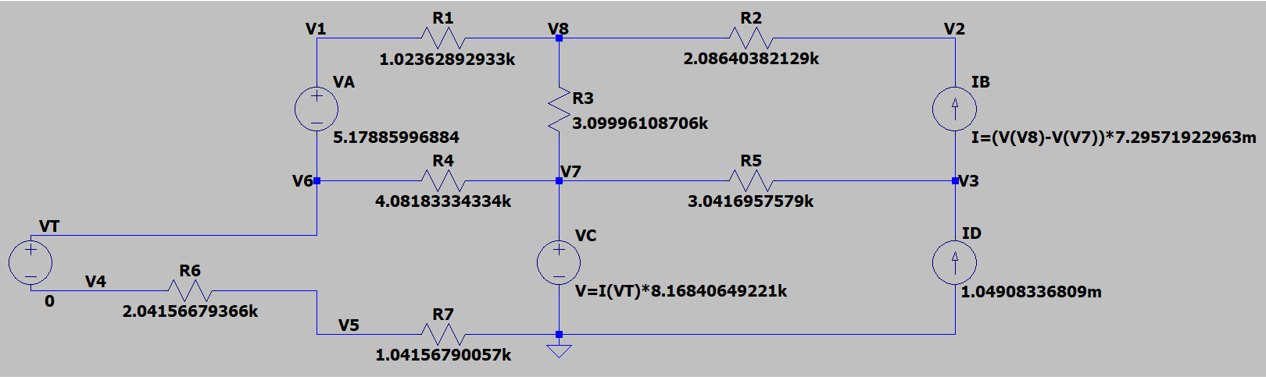
\includegraphics[width=0.8\linewidth]{CircuitLTSpice.png}
    \centering
    \caption{Circuit represented through \textit{LTSpice}}
    \label{circuitsim}
\end{figure}

\par $V_T$ is set to 0 meaning it will function as an ammeter. This is strictly for the purpose of the simulation. In the \textit{Spice} language, in particular in the \textit{NGSpice} software, for a current-controled voltage source there is an input that requires the current, which is controling the voltage source. We can measure that current by inserting an independent voltage source set to 0, making it possible to determine the current that is flowing in that branch without disturbing the system.
The $V_T$ source will be connected to 2 nodes that have the same voltage ($V_6$ and $V_4$), so, although both nodes are used in the simulation, for theoretical analysis one of them was supressed. For coherence purposes it was decided that the same numeration would be used in all models, so we decided to supress $V_4$, therefore not showing it in any analysis.


\par Running the simulation with \textit{NGSpice} we obtained the following results shown in Table~\ref{tab:op}. 

\begin{table}[H]
  \centering
  \begin{tabular}{|l|r|}
    \hline    
    {\bf Name} & {\bf Value [A or V]} \\ \hline
    \input{../sim/op_tab}
  \end{tabular}
  \caption{Operating point. A variable preceded by @ is of type {\em current}
    and expressed in Ampere; other variables are of type {\it voltage} and expressed in
    Volt.}
  \label{tab:op}
\end{table}

\par The data provided by the simulation is enough to solve all the circuit.
That being said, some values need some work so they can be compared. For instance, $V_7$ can be associated  to $V_c$, because $V_c$ imposes the voltage between the ground and $V_7$ implying that $V_7$ equals to $V_c$. $V_a$ is known data, therefore no calculations are executed. Also:

\begin{equation}
	V_b=V_{8}-V_{7}
\end{equation}

\par For the calculations of the currents we can assume that $I_{R_{1}}$ and $I_{R_{6}}$ are equal to $I_a$ and $I_c$, respectively. The current $I_b$ is the current in "g1", the voltage-controlled current source. Once again $I_d$ is a known data.
\par Due to linearity of the resistors, all voltages and currents can be determined knowing the resistance of the resistors, which is given.
\par Finally we can say the circuit has been solved and the results are the following:
\begin{table}[H]
    \centering
    \begin{tabular}{|c|c|}
    \hline
        $I_a$ & 2.40136e-04\\ \hline
        $I_b$ & 2.51245e-04\\ \hline
        $I_c$ & 9.76838e-04\\ \hline
        $V_b$ & 3.4437e-02\\ \hline
        $V_c$ & 7.979210e+00\\ \hline
    \end{tabular}
    \caption{Table of results for the simulation in A and V}
\end{table}









\newpage{}

\section{Conclusion}
\label{sec:conclusion}
\paragraph{}
\par Starting the conclusion with a comparison between Octave and NGSpice values, the results are as follows:
\begin{table}[H]
	\begin{minipage}{.5\linewidth}
		\centering
		\begin{tabular}{|c|c|}
		\hline
		\input{../mat/Comp.tex}
		\end{tabular}
		\caption{Theoretical Analysis}
		\label{ta}
	\end{minipage}
	\begin{minipage}{.5\linewidth}
		\centering
		\begin{tabular}{|c|c|}
		\hline
		\input{../sim/zin_TAB.tex}
    		\input{../sim/zo_TAB.tex}
    		\input{../sim/sim_TAB.tex}
	\end{tabular}
		\caption{Simulation Analysis}
		\label{sa}
	\end{minipage} 
\end{table}


\begin{figure}[H]
\centering
\begin{subfigure}{.5\textwidth}
  \centering
  \includegraphics[width=.75\linewidth]{gain.eps}
  \caption{Theoretical Analysis}
  \label{fig:sim4}
\end{subfigure}%
\begin{subfigure}{.5\textwidth}
  \centering
  \includegraphics[width=.60\linewidth]{../sim/gain.pdf}
  \caption{Simulation Analysis}
  \label{fig:sim5}
\end{subfigure}
\end{figure}





\begin{figure}[H]
\centering
\begin{subfigure}{.5\textwidth}
  \centering
  \includegraphics[width=.75\linewidth]{phase.eps}
  \caption{Theoretical Analysis}
  \label{fig:sim4}
\end{subfigure}%
\begin{subfigure}{.5\textwidth}
  \centering
  \includegraphics[width=.60\linewidth]{../sim/phase.pdf}
  \caption{Simulation Analysis}
  \label{fig:sim5}
\end{subfigure}
\end{figure}
		

\par It is clear just from looking at the information above that the model done is fairly accurate in both scenarios, with every aspect being very similar with the exception of both plots, more noticeably for the frequency response phase. This particular discrepancy can be explained by the non-linearity of the circuit, a problem present in every lab assignment with components with that behaviour, or the fact that the OpAmp used in the theoretical analysis was an ideal one with no output impedance and infinte output impedance, whereas in the simulation a more specific and complex model is used.
\par To wrap it all up, the objective of this laboratory was successfully completed, obtaining a merit of 1.49519e-5.


















%\cleardoublepage

% ----------------------------------------------------------------------
%  Bibliography
% ----------------------------------------------------------------------
%\addcontentsline{toc}{section}{\bibname}
%\bibliographystyle{abbrvunsrtnat} % <<<<< SELECT IF USING REFERENCES BY NUMBER (CITATION ORDER)
%\bibliography{../../../BIBfile.bib}

% ----------------------------------------------------------------------
\end{document}
% ----------------------------------------------------------------------
